% The LisaFlow network (src/canna/lisa/network.py, networks/mmdit.py), as a standalone
% figure. Build: pdflatex architecture.tex, then copy the pdf to ../architecture.pdf
\documentclass[tikz,border=2pt]{standalone}
\usepackage[T1]{fontenc}
\usepackage{tgheros}
\renewcommand{\familydefault}{\sfdefault}
\usepackage[italic]{mathastext}
\usepackage{amssymb}
\usetikzlibrary{positioning,fit,arrows.meta,calc,backgrounds}

% the figures' palette: blue for the parameter stream, a warm grey for the data stream
\definecolor{ink}{HTML}{0B0B0B}
\definecolor{ink2}{HTML}{52514E}
\definecolor{muted}{HTML}{898781}
\definecolor{xfill}{HTML}{CDE2FB}
\definecolor{xline}{HTML}{2A78D6}
\definecolor{yfill}{HTML}{F0EFEC}
\definecolor{yline}{HTML}{898781}
\definecolor{cfill}{HTML}{FFFFFF}

\begin{document}
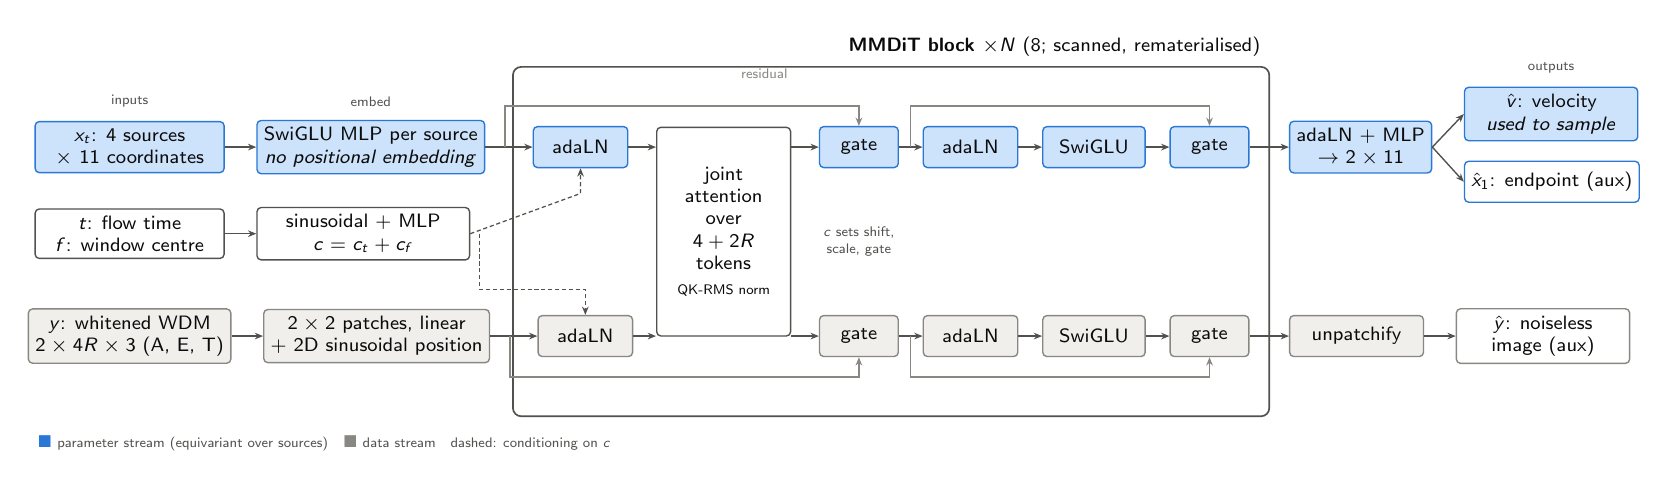
\begin{tikzpicture}[
    font=\scriptsize, text=ink, >={Stealth[length=3pt,width=2.4pt]},
    box/.style={draw=#1, rounded corners=1.5pt, line width=0.5pt, align=center,
                inner sep=2.5pt, minimum height=5.2mm},
    xbox/.style={box=xline, fill=xfill},
    ybox/.style={box=yline, fill=yfill},
    cbox/.style={box=ink2, fill=cfill},
    lbl/.style={font=\tiny, text=ink2, align=center},
    arr/.style={->, line width=0.5pt, draw=ink2},
    carr/.style={->, line width=0.45pt, draw=ink2, dashed, dash pattern=on 1.5pt off 1pt},
  ]

  % ---- inputs
  \node[xbox, minimum width=24mm] (xin) at (0, 1.55) {$x_t$: 4 sources\\ $\times$ 11 coordinates};
  \node[cbox, minimum width=24mm] (tin) at (0, 0.45) {$t$: flow time\\ $f$: window centre};
  \node[ybox, minimum width=24mm] (yin) at (0, -0.85) {$y$: whitened WDM\\ $2\times 4R\times 3$ (A, E, T)};
  \node[lbl, above=0.5mm of xin] {inputs};

  % ---- embeddings
  \node[xbox, minimum width=27mm, right=4mm of xin] (xemb) {SwiGLU MLP per source\\ \textit{no positional embedding}};
  \node[cbox, minimum width=27mm, right=4mm of tin] (temb) {sinusoidal + MLP\\ $c = c_t + c_f$};
  \node[ybox, minimum width=27mm, right=4mm of yin] (yemb) {$2\times2$ patches, linear\\ + 2D sinusoidal position};
  \node[lbl, above=0.5mm of xemb] {embed};
  \draw[arr] (xin) -- (xemb);
  \draw[arr] (tin) -- (temb);
  \draw[arr] (yin) -- (yemb);

  % ---- backbone: one block drawn in full, repeated N times
  \coordinate (b0) at ($(xemb.east)+(6mm,0)$);
  \node[xbox, minimum width=12mm, right=6mm of xemb] (xmod1) {adaLN};
  \node[ybox, minimum width=12mm, right=6mm of yemb] (ymod1) {adaLN};
  \node[box=ink2, fill=white, minimum width=17mm, minimum height=26.5mm, align=center,
        right=3.5mm of xmod1.east, anchor=north west, yshift=2.6mm] (att)
        {joint\\ attention\\ over\\ $4+2R$\\ tokens\\[1pt] {\tiny QK-RMS norm}};
  \node[xbox, minimum width=10mm, right=3.5mm of att.east |- xmod1] (xg1) {gate};
  \node[ybox, minimum width=10mm, right=3.5mm of att.east |- ymod1] (yg1) {gate};
  \node[xbox, minimum width=12mm, right=3mm of xg1] (xmod2) {adaLN};
  \node[ybox, minimum width=12mm, right=3mm of yg1] (ymod2) {adaLN};
  \node[xbox, minimum width=13mm, right=3mm of xmod2] (xmlp) {SwiGLU};
  \node[ybox, minimum width=13mm, right=3mm of ymod2] (ymlp) {SwiGLU};
  \node[xbox, minimum width=10mm, right=3mm of xmlp] (xg2) {gate};
  \node[ybox, minimum width=10mm, right=3mm of ymlp] (yg2) {gate};

  \draw[arr] (xemb) -- (xmod1);
  \draw[arr] (yemb) -- (ymod1);
  \draw[arr] (xmod1) -- (xmod1 -| att.west);
  \draw[arr] (ymod1) -- (ymod1 -| att.west);
  \draw[arr] (xg1 -| att.east) -- (xg1);
  \draw[arr] (yg1 -| att.east) -- (yg1);
  \draw[arr] (xg1) -- (xmod2);
  \draw[arr] (yg1) -- (ymod2);
  \draw[arr] (xmod2) -- (xmlp);
  \draw[arr] (ymod2) -- (ymlp);
  \draw[arr] (xmlp) -- (xg2);
  \draw[arr] (ymlp) -- (yg2);

  % residual connections, above the x lane and below the y lane
  \draw[arr, draw=muted] ($(xemb.east)+(2.5mm,0)$) -- ++(0,5.2mm) -| ($(xg1.north)$);
  \draw[arr, draw=muted] ($(xg1.east)+(1.5mm,0)$) -- ++(0,5.2mm) -| ($(xg2.north)$);
  \draw[arr, draw=muted] ($(yemb.east)+(2.5mm,0)$) -- ++(0,-5.2mm) -| ($(yg1.south)$);
  \draw[arr, draw=muted] ($(yg1.east)+(1.5mm,0)$) -- ++(0,-5.2mm) -| ($(yg2.south)$);
  \node[lbl, text=muted] at ($(xg1.north)+(-12mm,6.6mm)$) {residual};

  % the conditioning vector modulates every adaLN and gate
  \coordinate (cbus) at ($(temb.east)+(1mm,0)$);
  \draw[carr] (temb.east) -- ($(xmod1.south)+(0,-3.2mm)$) -- (xmod1.south);
  \draw[carr] ($(temb.east)+(1.2mm,0)$) |- ($(ymod1.north)+(0,3.2mm)$) -- (ymod1.north);
  \node[lbl] at ($(xg1.south)!0.5!(yg1.north)$) {$c$ sets shift,\\ scale, gate};

  % the block frame
  \begin{scope}[on background layer]
    \node[draw=ink2, rounded corners=3pt, line width=0.6pt, fill=white,
          fit=(xmod1)(ymod1)(att)(xg2)(yg2), inner xsep=2.5mm, inner ysep=7.5mm] (block) {};
  \end{scope}
  \node[font=\scriptsize\bfseries, anchor=south east] at (block.north east)
        {MMDiT block $\times N$ \normalfont(8; scanned, rematerialised)};

  % ---- heads
  \node[xbox, minimum width=17mm, right=5mm of xg2] (xhead) {adaLN + MLP\\ $\to 2\times 11$};
  \node[ybox, minimum width=17mm, right=5mm of yg2] (yhead) {unpatchify};
  \draw[arr] (xg2) -- (xhead);
  \draw[arr] (yg2) -- (yhead);
  \node[xbox, minimum width=22mm, right=4mm of xhead, yshift=4.2mm] (vout) {$\hat v$: velocity\\ \textit{used to sample}};
  \node[xbox, minimum width=22mm, right=4mm of xhead, yshift=-4.4mm, fill=white] (x1out) {$\hat x_1$: endpoint (aux)};
  \node[ybox, minimum width=22mm, right=4mm of yhead, fill=white] (yout) {$\hat y$: noiseless\\ image (aux)};
  \draw[arr] (xhead.east) -- (vout.west);
  \draw[arr] (xhead.east) -- (x1out.west);
  \draw[arr] (yhead) -- (yout);
  \node[lbl, above=0.5mm of vout] {outputs};

  % legend of the two streams
  \node[lbl, anchor=north west] at ($(yin.west |- block.south)+(0,-1.2mm)$)
        {\textcolor{xline}{$\blacksquare$} parameter stream (equivariant over sources)\quad
         \textcolor{yline}{$\blacksquare$} data stream\quad
         dashed: conditioning on $c$};
\end{tikzpicture}
\end{document}
